\documentclass[10pt,twocolumn,letterpaper]{article}

\usepackage{cvpr}
\usepackage{times}
\usepackage{epsfig}
\usepackage{graphicx}
\usepackage{amsmath}
\usepackage{amssymb}
\usepackage{wrapfig}
%\usepackage{subfig}
\usepackage{rotating}
\usepackage{multirow}
\usepackage{graphicx}
\usepackage{caption}
\usepackage{subcaption}
%\usepackage[usenames,dvipsnames]{color}
% Include other packages here, before hyperref.

% If you comment hyperref and then uncomment it, you should delete
% egpaper.aux before re-running latex.  (Or just hit 'q' on the first latex
% run, let it finish, and you should be clear).
\usepackage[pagebackref=true,breaklinks=true,letterpaper=true,colorlinks,bookmarks=false]{hyperref}


%\cvprfinalcopy % *** Uncomment this line for the final submission

\def\cvprPaperID{39} % *** Enter the CVPR Paper ID here
\def\httilde{\mbox{\tt\raisebox{-.5ex}{\symbol{126}}}}

% Pages are numbered in submission mode, and unnumbered in camera-ready
\ifcvprfinal\pagestyle{empty}\fi

%%%%%%%%% TITLE
\title{\vspace{-5ex}Using humans to build mid-level features\vspace{-3ex}}
\author{Genevieve Patterson\textsuperscript{1} \quad Tsung-Yi Lin\textsuperscript{2} \quad James Hays\textsuperscript{1}\\
 Brown University\textsuperscript{1} \quad University of California, San Diego\textsuperscript{2}}



\begin{document}
% \thispagestyle{empty}
\maketitle
%%%%%%%%% ABSTRACT
\begin{abstract}
  Identifying the distinctive parts of an image is a challenging task for computer vision. In contrast to previous methods, we use human participants to discover mid-level discriminative features. Amazon Mechanical Turk (AMT) workers filter groups of patches to identify clusters that have strong visual and semantic similarity.  We show that SVMs trained from human-defined discriminative patches outperform that patch classifiers discovered by Singh et al. and Doersch et al. \cite{singh2012unsupervised, doersch2012makes} when used as features for classification on the 15 scene dataset \cite{lazebnik2006beyond}.

\end{abstract}

\section{Introduction}
%Section 1, Intro:
%(1) Discriminative patches are hot. \cite{singh2012unsupervised, doersch2012makes, juneja13blocks}
%(2) They have demonstrated state of the art performance for various recognition tasks. [examples, citations].
%(3) What is the big idea behind these representations? How do they relate to bag of words models?
%(4) While there are several proposed methods to discover discriminative patches [examples, citations], we examine an interesting alternative -- having non-expert humans-in-the-loop to tell us which visual elements they think are discriminative. 
%
%(5) Relation to other human-in-the-loop methods \cite{gingold2012micro, branson2010visual, kovashka2012whittlesearch},. Humans (possibly non expert, crowdsourced humans) are commonly used in vision algorithms at two stages (a) annotation time, either exhaustively annotating a dataset or providing the most informative annotations in an "active learning" framework or (b) test time, coupled with a computational method (e.g. visipedia) to improve human accuracy and / or reduce human effort. In contrast, we put humans in the loop at neither annotation time or test time, but rather at "representation discovery" time. The humans are directly telling the computer which visual elements should be discriminative. This has some similarity to part-based annotation of visual phenomena, except we don't require any explicit semantic meaning for the parts, and in our initial experiments the humans never even see entire images. Putting humans "in the loop" at this stage in a recognition algorithm, is, to the best of our knowledge, never before studied.

Recently, several publications have demonstrated state of the art performance at scene classification using discriminative patches \cite{singh2012unsupervised, doersch2012makes, juneja13blocks}. These papers introduce different methods for identifying salient visual elements in the form of mid-sized image patches,  and training classifiers to detect the visual phenomena observed in training patches. Singh et al. and Juneja et al. each propose pipelines for training discriminative patch classifiers, but both employ a library of discovered patches to create ``bags of parts'' for scene classification. The methods shown in \cite{singh2012unsupervised, juneja13blocks} show state of the art performance compared to other single features on the MIT Scene 67 dataset. Doersch et al. shows impressive capability to discriminate between the architecture of different European cities. 

The insight of these papers is that scene and object categories can be separated from each other by observing a small number of visual events that are highly discriminative. Unlike bag of words models, not all of the locations are equally discriminative -- only a sparse set of locations in an image are useful for determining the category. Detectors trained on discriminative patches can build features that are more useful for scene classification than directly using low-level features. This would be similar to identifying only the most discriminatively powerful visual words, and only using those words in the bag of words codebook. Patches also have the advantage of being larger than the typical visual word, thus enabling them to capture a visual element that could have higher-level semantic significance. 

While there are several proposed methods to discover discriminative patches, \cite{singh2012unsupervised, juneja13blocks}, we examine an interesting alternative to the often time consuming methods of automatic discriminative patch discovery. We directly ask non-expert humans to select visually and semantically similar image patches. We train classifiers to recognize the human-identified visual elements. 
%Our motivation stems from the observation that humans are capable of rapidly discriminating scenes, and thus can be considered an upper bound on identifying which elements of scenes are the most salient.

Other human-in-the-loop methods such as \cite{gingold2012micro, branson2010visual, kovashka2012whittlesearch} have demonstrated success at visual classification tasks. Humans (often non-expert, crowdsourced humans) are commonly used in vision algorithms at two stages (a) annotation time, either exhaustively annotating a dataset or providing the most informative annotations in an ``active learning" framework or (b) test time, coupled with a computational method to improve human accuracy and / or reduce human effort. In contrast, we put humans in the loop at neither annotation time nor test time, but rather at ``representation discovery" time. The humans are directly telling the computer which visual elements should be discriminative. This has some similarity to part-based annotation of visual phenomena, except that our method does not require any explicit semantic meaning for the parts. In our experiments the humans never even see entire training images, only sets of candidate image patches. Putting humans ``in the loop" at this stage in a recognition algorithm is to the best of our knowledge unexplored.

\section{Building Human Patches}
%Section 2, Approach:
%More specifics about our starting point (CMU method), and how we put humans in the loop, and how we learn from human annotations, and how the human-based learning compares to the cross-validation-based learning (which is probably the most complicated, most accurate way to learn these models)
%
%How do we actually turn the human filtering into discriminative patch classifiers? One classifier per HIT? Or have a stronger requirement on consensus?
%
%What if the human filtered patches are consistent concepts, but they're not close enough together in the feature space? Can we do an optimization to translate (or rotate, or scale) each example in order to maximize their similarity in feature space before training the classifier? Can we train a non-linear classifier?

Our starting point for building human-in-the-loop patches is the automatic method presented in Singh et al. We first find candidate patches within the 15 scene dataset \cite{lazebnik2006beyond} using the code of \cite{singh2012unsupervised, doersch2012makes}. The algorithm selects a 1200 random patches from each category and for each patch finds its 24 nearest neighbors. Each random patch and its nearest neighbors are a candidate discriminative patch model. Individual patches are 80x80 pixel windows represented as 2112 dimensional HoG features.

At this point the Singh et al. use an iterative cross-validation method to discover sets of 5 patches that when used to train a linear SVM result in discriminatively powerful classifiers. Instead of this computationaly expensive process, we present AMT workers with a page showing a group of 25 nearest neighbor patches. We create a patch selection task for 400 randomly selected patch groups from each category in the 15 scene dataset. Our user interface is shown in Fig. \ref{fig:ui}.

%- user interface - 
\begin{figure}
\centering
 \includegraphics[width=0.4\textwidth]{cluster_ui2.png}
 \caption{\small \textit{AMT patch cluster refinement interface.} Users are presented with a group of 25 nearest neighbor patches. These user-selected patches are used to train a model for a discriminative patch. }
\vspace{-4mm}
 \label{fig:ui}
\end{figure}

%\begin{figure}
%\centering
% 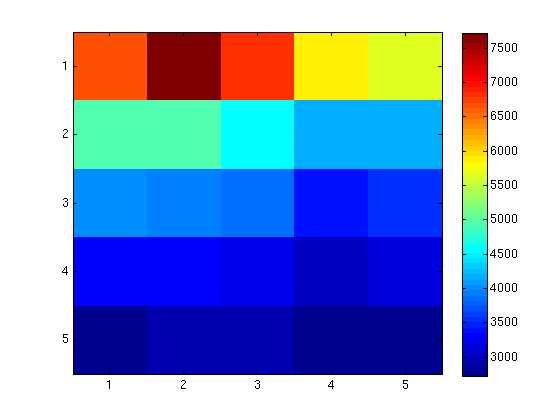
\includegraphics[width=0.3\textwidth]{votes_ui_patch_pos.png}
%\caption{This is the popularity of images in the corresponding positions on the UI. People often select the first image and it's 4 nearest neighbors.}
%\end{figure}
% - example patches auto and human X
%\begin{figure}
%\centering
% \includegraphics[width=0.3\textwidth]{high_ranked_patches.pdf}
% \caption{\small \textit{Most confident detections by Discriminative Patches on a test set from the 15 scene dataset.} Each row shows the top 5 most confident detections for a discriminative patch discovered for the listed scene category. For the automatically discovered patches, the detections shown are for the highest ranked patch for that category. Automatically discovered patches are ranked using the posterior ranking described in \cite{singh2012unsupervised}. The example detections shown for the human discovered patches are from patches selected at random from all of the discriminative patches discovered for that category.}
%\vspace{-4mm}
% \label{fig:ex_patches}
%\end{figure}

Using the interface in Fig. \ref{fig:ui}, we obtain 3 user responses for each nearest neighbor group.
%The user responses came in the form of a list of 5 or more patches from that group that the user considered to be visually similar. 
We discard redundant responses where the selected patches are nearly the same and train discriminative patch models from the remaining responses. For each discriminative patch classifier, the user selected patches are the positive examples and a large set of randomly selected patches from other categories are the negative examples.

%We obtain consensus responses from the raw data in the following manner: if two or more users agree that 3 or more patches are visually coherent, that group of 3 or more patches forms the training set for a discriminative patch model. If a user selects a set of patches that intersect by 2 or fewer patches with their colleagues' responses, we consider that the user has identified an independent visual phenomena and use that response to train a new discriminative patch classifier. 

%In the algorithm used for automatic patch discovery in \cite{singh2012unsupervised}, the models for the discriminative patches were trained using linear SVMs. Because the pipeline for building patch models from human responses was so much shorter, we trained the models using linear SVM and sigmoid SVMs.

After all of the discriminative patches for one of the 15 scene categories are identified, we also use a different method than \cite{singh2012unsupervised} to select which discriminative patches to use in our feature library. Singh et al. suggest ranking the output discriminative patches by the posterior probability that a given patch will fire in the category from which it was discovered. We use this method to create the features used in Fig. \ref{fig:results}. Instead of ranking the human patches, we simply selected them at random from the available library of patches discovered from the human responses. No ranking was used for the human patches.

\section{Results for Scene Classification}
Figure \ref{fig:results} shows the performance of scene classification on the 15 scene dataset using automatically discovered and human-in-the-loop discriminative patch models. In the case of human-in-the-loop patches, we tried both linear and non-linear SVM patch classifiers. Each set of discriminative patch classifier generates a ``bag of parts'' histogram for every image which encodes how often a particular patch was found. A second SVM is trained to classify images into scene categories based on these ``bags of parts''.  We set a detection threshold at a confidence of -1.0, as suggested in \cite{singh2012unsupervised}. An equal number of patches are selected from each scene category. Fig. \ref{fig:results} shows that the patches discovered using human intervention greatly outperform the automatically discovered patches for scene classification on the 15 scene dataset.

% - scene class acc X
\begin{figure}
\centering
% \begin{subfigure}[b]{0.45\textwidth}
% \centering
 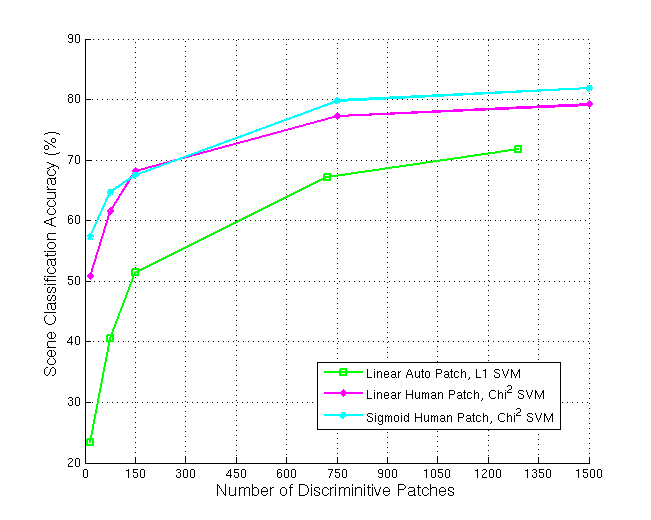
\includegraphics[width=0.45\textwidth, height=0.15\textheight]{perf.png}
 \caption{\small\textit{Scene Classification Performance of Human and Automatic Patches on the 15 scene dataset.}  Overall the sigmoid kernel human patches performs achieves the best performance at 81.89\% accuracy; the linear kernel human patches achieve 79.11\%, and the automatic patches top out at 71.82.}
\vspace{-4mm}
% \caption{\textit{Scene classification accuracy for the 15 scene dataset.} These trends show the increasing performance of scene classifiers trained on discriminative patch features of increasing dimensionality. Each trend line is the best performing type of scene classifier for the type of discriminative patch listed. Different kernel types performed the most successfully for the automatic and human discovered patches. For comparison, SVM models for the human patches were trained using linear classifiers as were the automatic patches \cite{singh2012unsupervised}. We also trained the human patch classifiers using a sigmoid kernel, which resulted in patches that performed slightly better as features. In all cases the mid-level feature used for scene classification is a histogram of the number of times each patch fired. From right to left the feature is increasing in the number of patches used. An equal number of patches was selected from each scene category. For the automatic patches, there were not always an equal number of patches available for each category, due to the constraints of the automatic discover process. When an equal number were not available, all available patches are used.}
% \label{fig:perf}
% \end{subfigure}
%\begin{subfigure}[b]{0.45\textwidth}
% \centering
% 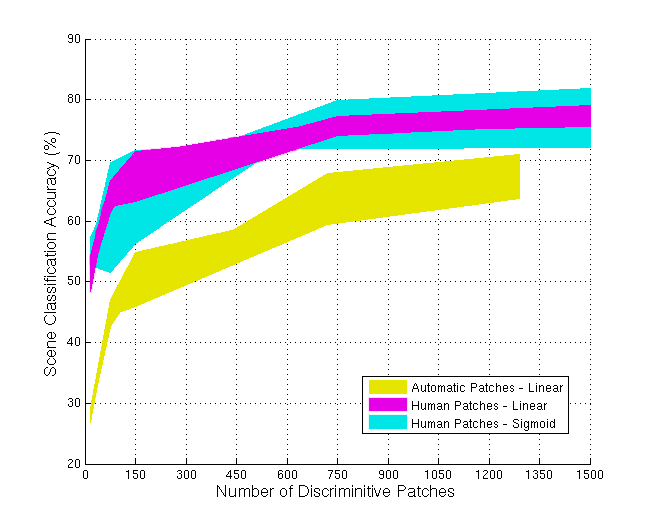
\includegraphics[width=\textwidth]{perf_overlay_graph.png}
% \caption{\textit{Range of scene classification accuracies for the 15 scene dataset using different kernel types.} The range of values for each color shown is the range of classification accuracies using L1, L2, $\chi^{2}$ and RBF kernels to train the scene category classifiers. Overall the sigmoid kernel human patches performs achieves the best performance at 81.89\% accuracy; the linear kernel human patches achieve 79.11\%, and the automatic patches top out at 71.82.}
% \label{fig:perf_overlay}
% \end{subfigure}

\label{fig:results}
\end{figure}
% - cat confusion comparison btwn auto and human. X
%\begin{figure}
%\centering
% 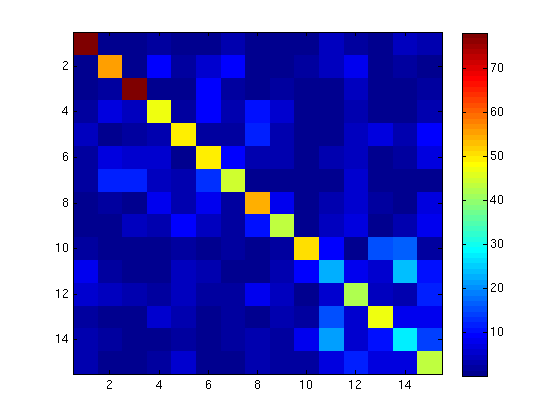
\includegraphics[width=0.5\textwidth]{scene_cat_confusion_auto_post_kchi2_10_patchespercat.pdf}
%\caption{Scene Category confusions using 150 automatic dpatches.}
%\end{figure}
%\begin{figure}
%\centering
% 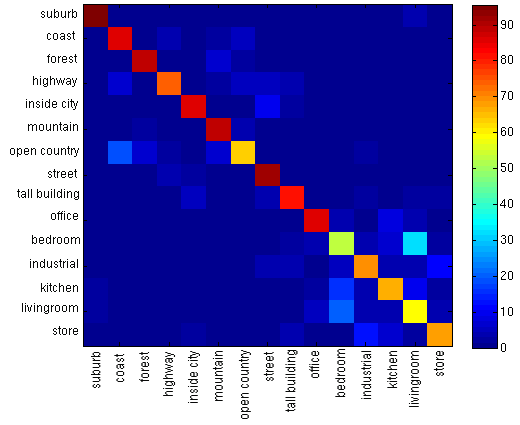
\includegraphics[width=0.5\textwidth]{scene_cat_confusion_human_kchi2_10_patchespercat.pdf}
%\caption{Scene Category confusions using 150 human dpatches.}
%\end{figure}


Interestingly, our human patch discovery method is arguably cheaper to implement than the automatic method. In our experience, it took 300 CPU hours plus 1200 AMT Human Intelligence tasks to discover patches for one scene category. It took us roughly 6000 CPU hours to automatically discover discriminative patches for one category. Using the default cost of an Amazon AWS instance (\$0.06 per instance per hour) and the cost of our AMT HITs (\$0.04 per HIT), it would cost \$66 to discover the human patches and \$360 to discover the automatic patches for one of the 15 scene categories. In light of the efficiency and accuracy shown by human patch discovery, we believe that using humans to build mid-level patches deserves further inquiry.

%\textbf{Acknowledgements.} We thank Hari Narayanan (Brown Univ.) for his insights and contributions in the data annotation process. Genevieve Patterson is supported by the Department of Defense (DoD) through the National Defense Science \& Engineering Graduate Fellowship (NDSEG) Program. This work is also funded by NSF CAREER Award 1149853 to James Hays. 

{\footnotesize
\bibliographystyle{ieee}
\bibliography{dpatch}
}

\end{document}
